%!TEX root = ../crimson_throne_book_main.tex
% 2015-06-30
The heroes have located the lizardfolk settlement in the Mistmoors. As they approach, they notice that the scaly creatures are all distracted by something:\hyperref[fig:Mistmoor-lizardfolk-sacrificing-centaur-543065415]{ they are all staring in the direction of the beating drum } . Balian seizes the opportunity to glide the boat right up to the pile huts. Puk jumps out of the boat and climbs the first building they pass, while Quint calls out with a friendly voice: "Here, catch!" He throws then end of a rope to the closest lizardman. Surprised by the sudden arrival of armed pinkskins, the creature shouts out in a language none of the companions understands, grabs his club and starts bashing his shield with it vehemently. The entire tribe picks up his war cry and looks ready for battle. \\

\begin{figure}[h]
	\centering
	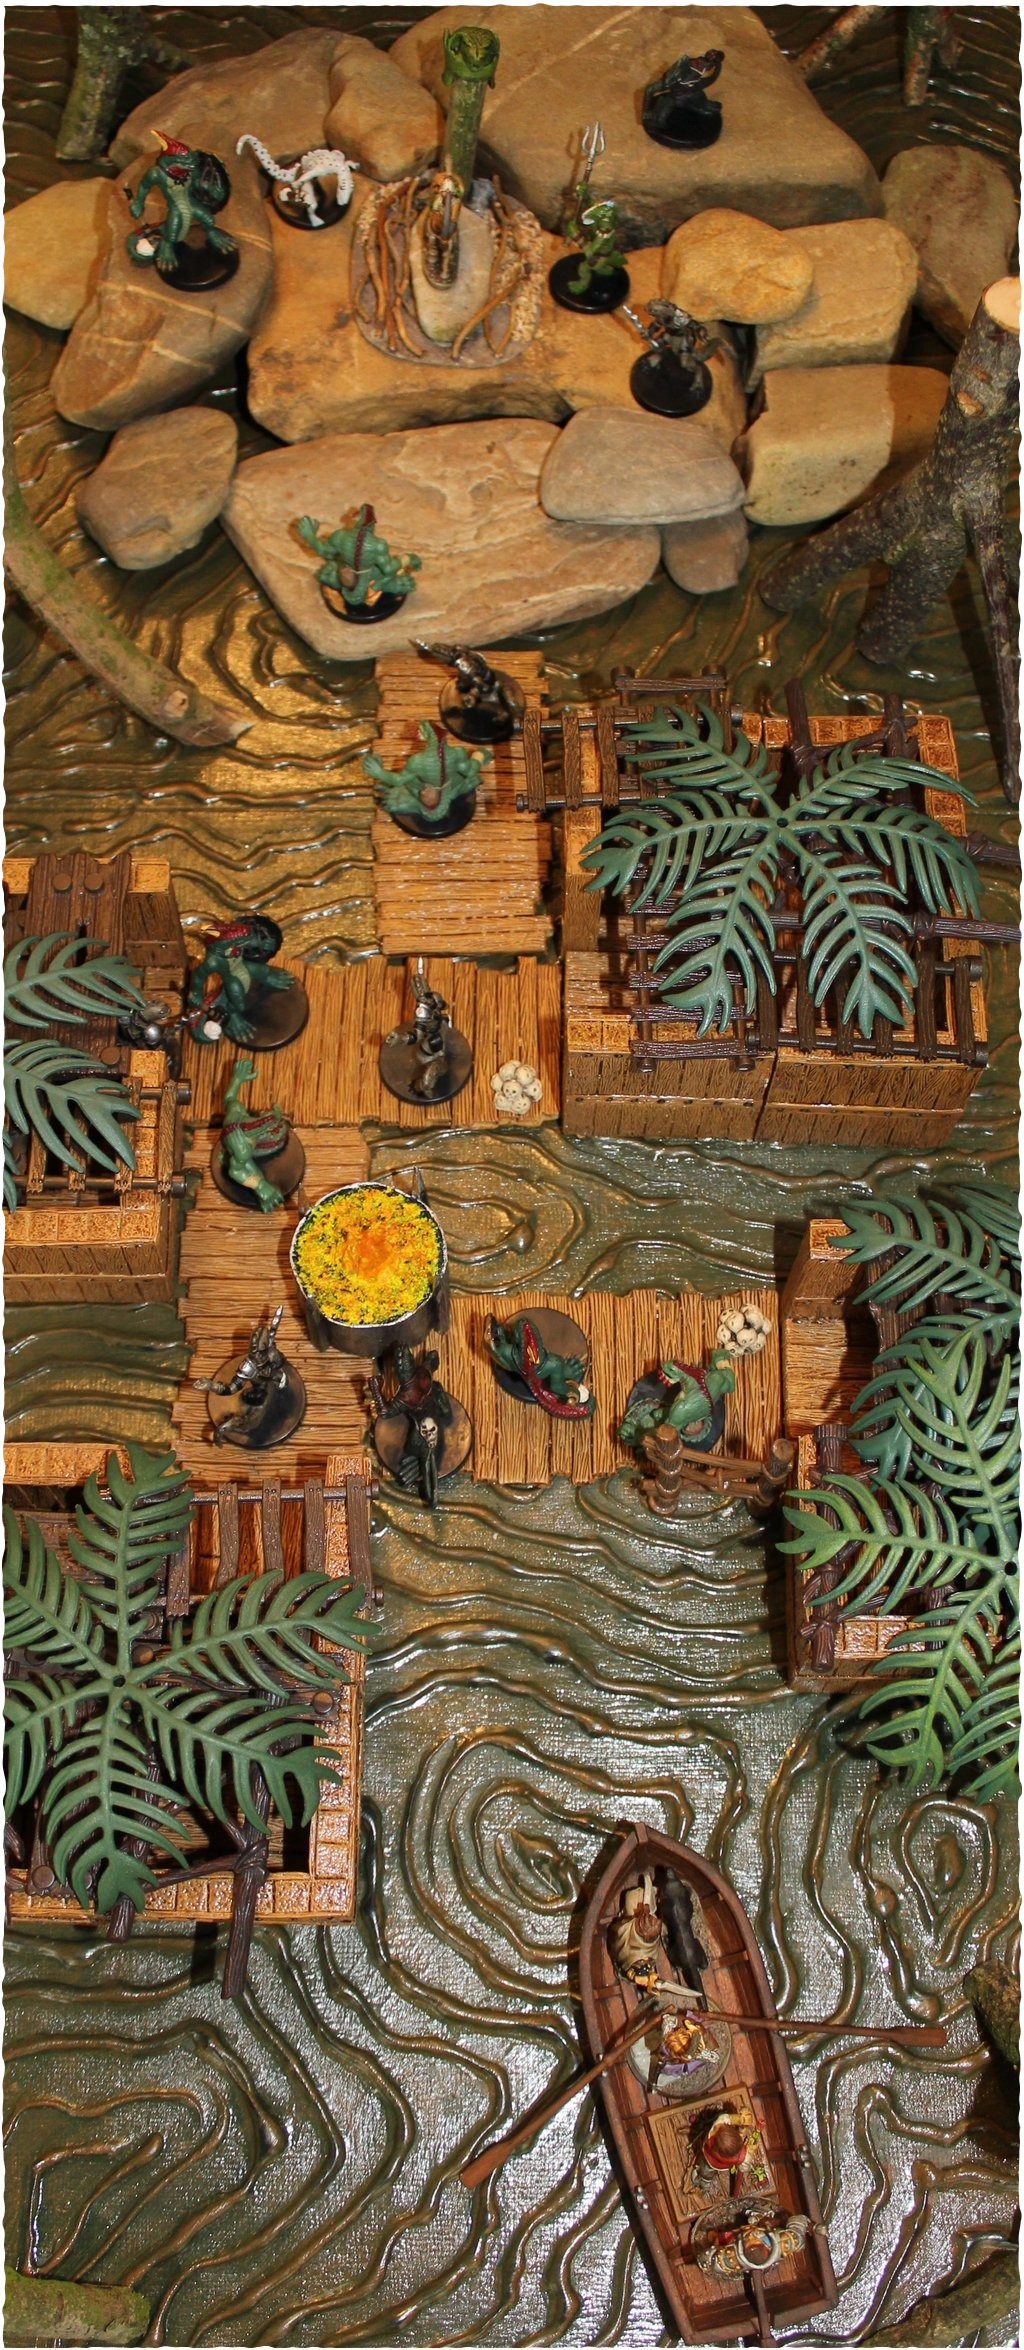
\includegraphics[width=0.4\textwidth]{images/Mistmoor-lizardfolk-sacrificing-centaur-543065415_mod.jpg}
	\caption{Mistmoor lizardfolk sacrificing centaur}
	\label{fig:Mistmoor-lizardfolk-sacrificing-centaur-543065415}
\end{figure}

While Quint realizes that he knows no language to successfully communicate with these creatures, his friends jump into battle and quickly take down a number of lizardfolk. Sjo notices a mass of rocks beyond the pile houses, where a fair number of scaly creatures have gathered. He summons a mighty fireball, killing four of them and wounded two others. Puk, Balian and Spyder meet with more resistance as they face some lizardmen wearing hide armor and shields, obviously warriors of some kind. Quint trips one of them and again the bard calls out for a seize-fire, but to no avail. By now the chieftain joins the fight, while the white-scaled shaman summons an owlbear to slow down the heroes' advance.\\

Quint attempts to capture the chief in a {\itshape cacophonous call} , but the creature is not affected, and Sjo fails to dispel the owlbear. Meanwhile Balian and Spyder pick off the last 'common' tribesmen, so only the chief, shaman and the summoned monster remain. The ranger feels that the shaman tries to freeze him in place, but bites back and resists the  {\itshape hold person} . Quint finally manages to control the battlefield by nauseating the leader and his medicine man with two successful  {\itshape cacophonous calls} . Both of them slip into the murky waters, giving the companions the time to take out the owlbear and heal their wounds. Tied to some kind of sacrificial altar is Mirala, the missing centaur girl. Furian, the pixie, blinks out of invisibility and starts babbling away while Sjo unties the horsegirl. Mirala claims to be confused by the tribemen's behavior. They rescued her from the quicksand, took her to their village and treated her with respect, although she could not communicate with them. Today, they suddenly grabbed her and tied her to this pole, but she doesn't understand why. Sjo wonders if they were planning to bleed her out in a sacrificial ceremony, but Puk realizes they were literally trying to offer her to the creature that suddenly rears his ugly head from the swamp waters: a black dragon! Before they can react, the dragon spews a stream of biting acid on Sjo, Spyder, Quint and Furian. The little pixie goes down. Next the black-skinned retile sinks his teeth in Quint's flesh. At the same time the lizardfolk chieftain and shaman climb out of the water again. Puk and Sjo confront the dragon, while Balian and his dog fight back the two lizardmen. Quint distracts the enemies with his {\itshape satire} and hands his  {\itshape wand of cure serious wounds} to Mirala, who support the fight with some well-placed healing. During her medical work she sings an inspiring song which lightly boosts the companions fighting skills. Balian's greatsword cuts deeply into the chief's flesh, but his shaman sidekick heals him again. Fortunately, our ranger friend is on a roll and with a critical hit he takes down the fierce lizardman. The shaman flees into the water and swims to the dragon's side. This monster seems to have overestimated his own power: he does wound his opponents badly, but Mirala's healing keeps them on their feet and their weapons hit him time and again. The shaman heals him enough to continue fighting, but when Balian delivers another critical blow, the dragon decides not to tempt fate any longer and escapes, barely alive. The lizardfolk medicine man quickly follows his 'god', leaving the companions victorious. Sjo can bring back Furian from the brink of death, while Balian finds that the alter is covered in red toadstools: blood cap mushrooms! Hundreds of them!\\

